%%%%%%%%%%%%%%%%%%%%%%%%%%%%%%%%%%%%%%%%%%%%%%%%%%%%%%%%%%%%%%%%%%%
% Chapter 4: Numerical Experiment
%%%%%%%%%%%%%%%%%%%%%%%%%%%%%%%%%%%%%%%%%%%%%%%%%%%%%%%%%%%%%%%%%%%

\chapter{Numerical Experiment}
\label{chap:experiment}

% Chương 4 mô tả các thí nghiệm để đánh giá \verb|Temporal-ML| và so sánh với \verb|NHITS| trên các tập dữ liệu lớn và phổ biến. Các thí nghiệm được thực hiện trên aperiodic data bao gồm một dataset duy nhất và aperiodic data bao gồm nhiều datasets để kiểm chứng khả năng rút trích các thông tin về thị trường cũng như khả năng tổng hợp thông tin từ nhiều nguồn. Dữ liệu có chu kỳ cũng được sử dụng để tăng tính khách quan trong các đánh giá. Ngoài ra, chúng tôi thực hiện loại bỏ/thay thế các component của \verb|Temporal-ML| để phân tích kỹ khả năng của các components này.

Chapter 4 describes experiments to evaluate \verb|Temporal-ML| and compare it with \verb|NHITS| on large and popular datasets. The experiments are performed on aperiodic data consisting of a single dataset and aperiodic data consisting of multiple datasets to verify the ability to extract market information as well as the ability to aggregate information from multiple sources. Periodic data is also used to increase the objectivity of the evaluations. In addition, we perform the removal/replacement of components of \verb|Temporal-ML| to analyze the capabilities of these components in detail.

% ablation study
% Ngoài ra, so sánh giữa \verb|Temporal-ML| và các mô hình đơn lẻ \verb|LSTM|, \verb|LSTM+CNN| cũng được thực hiện như một ablation study.

\section{Dataset description}

% mô tả dữ liệu
% FX nói riêng và các chỉ số tài chính nói chung là dạng dữ liệu điển hình cho aperiodic time-series data. Do đó, chúng tôi chọn loại dữ liệu này để kiểm thử mô hình. Cụ thể, chúng tôi cấu hình hai bộ dữ liệu sử dụng dữ liệu FX. Bộ dữ liệu \verb|USD/JPY| chỉ gồm dữ liệu của cặp tiền tệ USD/JPY, được chia thành 60 tập dữ liệu con theo trình tự thời gian với kích thước bằng nhau. Dữ liệu được sample theo giờ từ năm 2000 đến năm 2024, bao gồm các thuộc tính open, low, high, và close price. Bộ dữ liệu \verb|multi-fx| bao gồm 60 cặp tiền tệ giữa 18 quốc gia Australia, Canada, Switzerland, Denmark, EU, United Kingdom, Hong Kong, Iceland, Japan, Norway, New Zealand, Singapore, Sweden, Turkey, United States, Mexico, China, South Africa. Dữ liệu có thuộc tính tương tự như \verb|USD/JPY| và được sample theo ngày từ năm 2014 đến 2024.

Foreign exchange in particular and financial indices in general are typical data types for aperiodic time-series data. Therefore, we choose this type of data to test the model. Specifically, we configure two datasets using foreign exchange data. \verb|USD/JPY| dataset consists of only data of the exchange rate between US dollar and Japanese yen. The data is sampled hourly from 2000 to 2024, including the attributes of open, low, high, and close price. \textbf{By carefully examining the transaction history as well as effectively aggregating data characteristics, we expect to forecast the movement of price without utilizing external information.}

\verb|multi-fx| dataset consists of 60 currency pairs made of 18 countries: Australia, Canada, Switzerland, Denmark, EU, United Kingdom, Hong Kong, Iceland, Japan, Norway, New Zealand, Singapore, Sweden, Turkey, United States, Mexico, China, South Africa. The data has similar attributes to \verb|USD/JPY| and sampled daily from 2014 to 2024. \textbf{By integrating analysis of multiple sources of information in the domain of FX, we expect to obtain valuable analytical insights for the indicator of interest.}

% Ngoài ra, chúng tôi sử dụng thêm 2 bộ dữ liệu: Electricity Transformer Temperature (\verb|ETT-m2|) và Weather (\verb|WTH|). Tập dữ liệu \verb|ETT-m2| bao gồm 7 trường dữ liệu, đo đạc các thông số của máy biến áp tại một tỉnh của Trung Quốc sau mỗi 15 phút trong khoảng thời gian từ July 2016 to July 2018. Tập dữ liệu \verb|WTH| bao gồm 12 trường dữ liệu, ghi nhận các thông số của thời tiết tại Weather Station of the Max Planck Biogeochemistry Institute in Jena, Germany sau mỗi 10 phút trong năm 2020. Đây là hai tập dữ liệu thể hiện tính chu kỳ rất mạnh mà \verb|NHITS| đã rất thành công trong việc dự đoán. Thực nghiệm trên chúng giúp so sánh toàn diện hơn về khả năng của phương pháp đề xuất đối với \verb|NHITS|.

In addition, we used two periodic datasets: Electricity Transformer Temperature (\verb|ETT-m2|) \cite{zhou2021informer} and Weather (\verb|WTH|) \cite{Kolle}. \verb|ETT-m2| dataset consists of 7 data fields, measuring the parameters of a transformer in a province of China every 15 minutes from July 2016 to July 2018. \verb|WTH| dataset consists of 12 data fields, recording the weather parameters at the Weather Station of the Max Planck Biogeochemistry Institute in Jena, Germany every 10 minutes in 2020. These two datasets exhibit very strong periodicity, which \verb|NHITS| has been very successful in predicting. Experiments on them provide a more comprehensive comparison of the proposed method's capabilities against \verb|NHITS|.

\section{Temporal-ML}

\subsection{Data pre-processing}
\label{subsec:ml_preprocess}

% viết về cách tổng hợp metric ở đây
% xét trên 1 thuộc tính cố định: chạy 60 thằng -> 60 bộ metric. lấy TBC trên 60 bộ này -> metric ± std
% chạy hết các attribute -> 4 thằng metric ± std
% -> trung bình theo kiểu mean(metric), \sqrt(mean(std^2))

% Như đã đề cập trong section \ref{sec:data_prep}, để sử dụng ML, các tập dữ liệu cần phải được cấu trúc thành các task riêng biệt. Trong mỗi task, tập support chiếm 20\% dữ liệu, tập query chiếm 80\% dữ liệu. Đối với \verb|multi-fx|, mỗi cặp tiền tệ được chia thành 2 tập dữ liệu, ứng với 2 tasks. Do đó, 60 cặp tiền tệ tạo thành 120 tasks. Đối với các tập dữ liệu còn lại, mỗi tập được chia nhỏ ra thành các chuỗi thời gian, mỗi chuỗi tương ứng với một task. Trong cả quá trình, 50\% số tasks được sử dụng trong quá trình meta-training, 25\% số tasks được sử dụng trong quá trình meta-validation, số tasks còn lại được sử dụng trong meta-testing. Thống kê dữ liệu cho các task theo tập dữ liệu được trình bày trong bảng \ref{tab:stat_}.

As mentioned in section \ref{sec:data_prep}, to use ML, the datasets need to be structured into separate tasks. In each task, the support set accounts for 20\% of the data, the query set accounts for 80\% of the data. For \verb|multi-fx|, each currency pair is divided into 2 datasets, corresponding to 2 tasks. Therefore, 60 currency pairs form 120 tasks. For the remaining datasets, each dataset is divided into time series, each corresponding to a task. During the whole process, 50\% of the tasks are used in the meta-training process, 25\% of the tasks are used in the meta-validation process, and the remaining tasks are used in meta-testing. Statistics for tasks by dataset are presented in table \ref{tab:stat_}.

\begin{table}[H]
    \centering
    \caption{Statistics on datasets.}
    \label{tab:stat_}
    \begin{tblr}{
        cells = {c},
        hline{1,6} = {-}{0.08em},
        hline{2} = {-}{},
    }
    Dataset                      & Attribute & Task & Sample    & Sample/Task    \\
    \Verb|USD/JPY|               & 4         & 60   & 150,175   & 2,503          \\
    \Verb|multi-fx|              & 4         & 120   & 154,440  & 1,287          \\
    \Verb|ETT-m2|                & 7         & 48   & 69,680    & 1,452          \\
    \Verb|WTH|                   & 12        & 40   & 35,064    & 877            
    \end{tblr}
\end{table}

% Vì các tập dữ liệu đều là time-series, dữ liệu trong quá trình huấn luyện không được tiết lộ bất cứ thông tin gì về tương lai. Do đó, 120 tasks của dữ liệu \verb|multi-fx| được chia như hình \ref{fig:multi_fx_split}. Đối với các tập dữ liệu còn lại, dữ liệu sử dụng trong quá trình huấn luyện, kiểm thử, kiểm tra phải đảm bảo thứ tự thời gian từ quá khứ đến tương lai.

Since the datasets are all time-series, the training data should not reveal any information about the future. Therefore, the 120 tasks of the \verb|multi-fx| dataset are divided as shown in \ref{fig:multi_fx_split}. For the remaining datasets, the data used in the training, testing, and validation must be in chronological order from past to future.

\begin{figure}[H]
    \centering
    \begin{subfigure}[b]{0.5\textwidth}
        \centering
        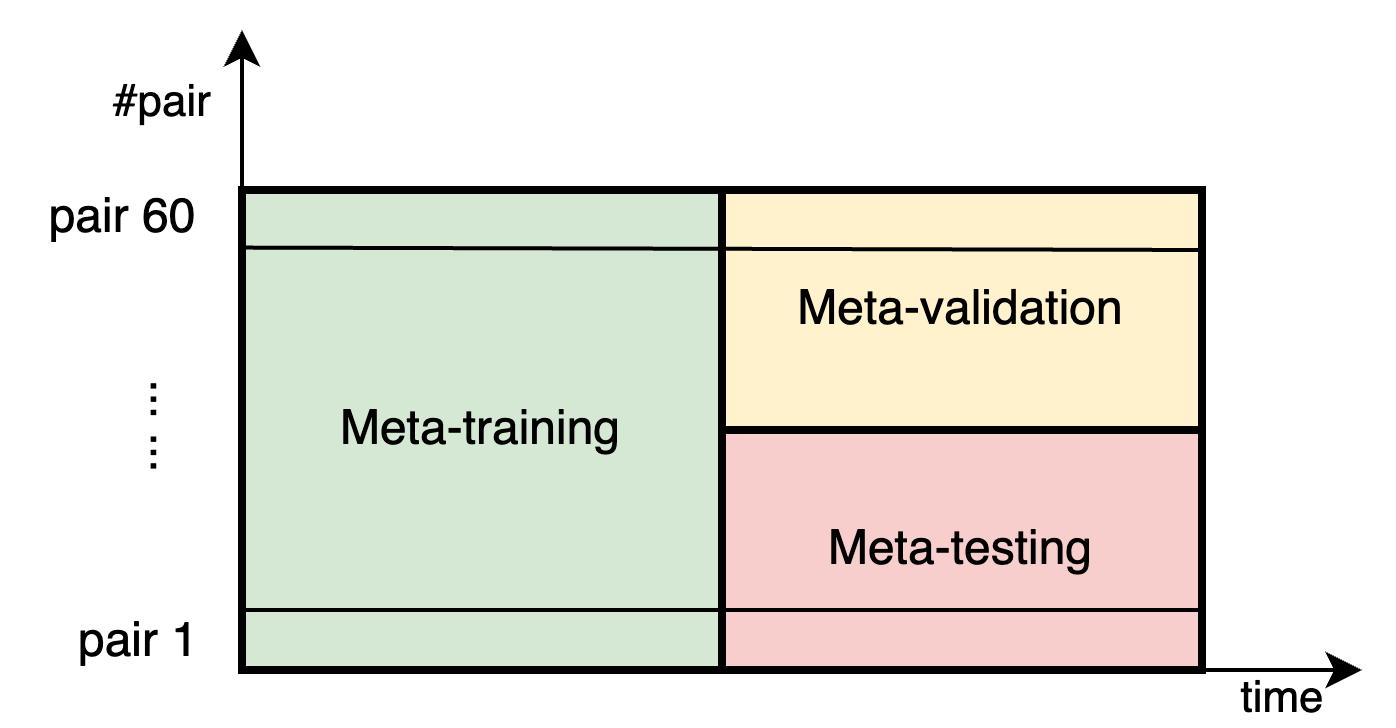
\includegraphics[width=\textwidth]{multi_fx.png}
        \caption{}
        \label{fig:multi_fx_split}
    \end{subfigure}%
    ~
    \begin{subfigure}[b]{0.5\textwidth}
        \centering
        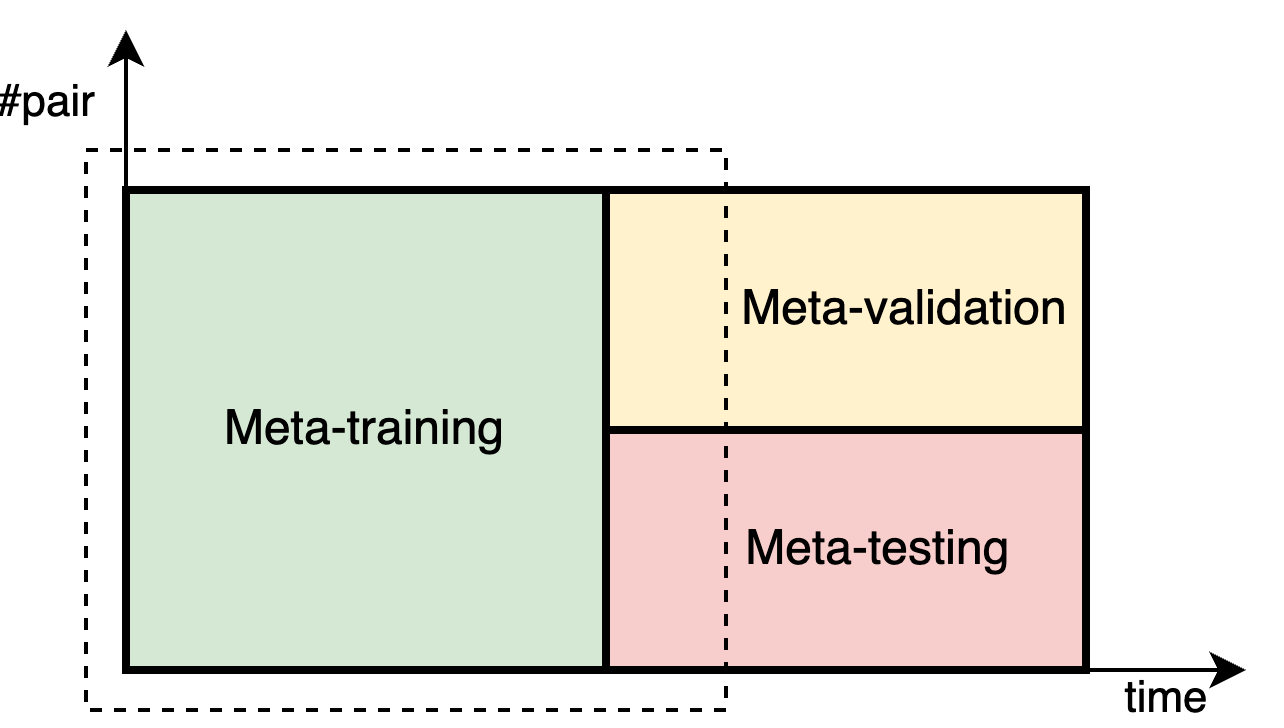
\includegraphics[width=0.92\textwidth]{multi_fx_prep.png}
        \caption{}
        \label{fig:multi_fx_prep}
    \end{subfigure}

    \cprotect\caption{(a): Splitting data for \verb|multi-fx|. (b): Pre-process for \verb|multi-fx| (dash line rectangle accounts for all training and 20\% data of validation and testing tasks).}
    % \label{fig:ill_aperiodic}
\end{figure}

% Quá trình tiền xử lý bằng \verb|z-score| theo đó được thực hiện trên toàn bộ dữ liệu huấn luyện và các tập support của dữ liệu kiểm thử và kiểm tra của từng cặp tiền tệ (see figure \ref{fig:multi_fx_prep}) vì đây là các dữ liệu đã được biết trước. Cụ thể, tiền xử lý thuộc tính $X$ được thực hiện như sau:

The \verb|z-score| preprocessing is then performed on the entire training data and the support sets of the test and validation data for each currency pair (see figure \ref{fig:multi_fx_prep}) since these are known data. Specifically, the preprocessing of attribute $X$ is performed as follows:

\begin{align}
    \mu_{X} &= \frac{1}{n} \sum_{i=1}^n{x_i} \quad \text{($n$ là số mẫu của thuộc tính $X$)} \label{eq:mean}\\
    \sigma_{X} &= \sqrt{\frac{1}{n} \sum_{i=1}^n{(x_i - \mu_X)^2}} \label{eq:std}\\
    X_{new} &= \frac{X - \mu_{X}}{\sigma_{X}} \label{eq:z_score}
\end{align}

% $\mu_{X}$ và $\sigma_{X}$ thu được từ phương trình \ref{eq:mean} và \ref{eq:std} được sử dụng để chuẩn hóa cho thuộc tính $X$ trong query set của quá trình meta-validation và meta-testing.

$\mu_{X}$ and $\sigma_{X}$ obtained from the equations \ref{eq:mean} and \ref{eq:std} are used to normalize the attribute $X$ in the query set of the meta-validation and meta-testing processes.

\subsection{Metric evaluation}

% Nghiên cứu sử dụng \textit{Accuracy, Precision, Recall}, và \textit{F1-score} để đánh giá các mô hình (equations \ref{eq:acc}, \ref{eq:P}, \ref{eq:R}, \ref{eq:F1}). Trong đó, \textit{Accuracy} được sử dụng để tính tỷ lệ giữa số mẫu phân lớp đúng và tổng số mẫu được dự đoán, \textit{Precision} đo mức độ tin cậy của mô hình khi nó gán nhãn cho một mẫu dữ liệu, \textit{Recall} kiểm định tỷ lệ bỏ sót các mẫu dữ liệu của một phân lớp, \textit{F1-score} kiểm tra mức độ bias của mô hình trên các nhãn có số lượng lớn bằng cách lấy trung bình điều hòa trên \textit{Precision} và \textit{Recall}.

The study uses \textit{Accuracy, Precision, Recall}, and \textit{F1-score} to evaluate the models (equations \ref{eq:acc}, \ref{eq:P}, \ref{eq:R}, \ref{eq:F1}). In which, \textit{Accuracy} is used to calculate the ratio between the number of correctly classified samples and the total number of predicted samples, \textit{Precision} measures the confidence level of the model when it labels a data sample, \textit{Recall} tests the rate of misclassified data samples of a classifier, \textit{F1-score} checks the level of bias of the model on major labels by taking the harmonic average over \textit{Precision} and \textit{Recall}.

\begin{align}
    acc &= \frac{TP+TN}{TP+FP+TN+FN}\label{eq:acc}\\
    P &= \frac{TP}{TP+FP}\label{eq:P}\\
    R &= \frac{TP}{TP+FN}\label{eq:R}\\
    F1 &= \frac{2PR}{P+R}\label{eq:F1}\\
\end{align}Where, $TP, TN, FP, FN$ are the number of \textit{true\_positive, true\_negative, false\_positive, false\_negative}, respectively.

% Giả sử thuật toán \verb|Temporal-ML| được đánh giá trên tập dữ liệu $\mathcal{D}$ gồm $a$ thuộc tính và được chia thành $n$ tasks. Quá trình đánh giá được thực hiện bằng cách để mô hình dự đoán xu hướng của từng thuộc tính với đầu vào là tất cả các thuộc tính, sau đó thực hiện hai bước tổng hợp: (1) - Tổng hợp trên task; (2) - Tổng hợp trên thuộc tính. Quá trình đánh giá này được thiết kế dựa trên \cite{challu2023nhits}.

Suppose the \verb|Temporal-ML| algorithm is evaluated on a dataset $\mathcal{D}$ consisting of $a$ attributes and divided into $n$ tasks. The evaluation is performed by letting the model predict the movement of each attribute with all attributes as input, then performing two aggregation steps: (1) - Aggregation on tasks; (2) - Aggregation on attributes. This evaluation process is designed based on \cite{challu2023nhits}.

% \textbf{Tổng hợp trên task}. Xét metric $m$ khi mô hình dự đoán thuộc tính $k$ bất kỳ ($1\leq k \leq a$). Sau khi dự đoán thuộc tính $k$, chúng ta thu được $n$ giá trị: $\{m^{(k)}_1,\dots,m^{(k)}_n\}$. Quá trình tổng hợp metrics $m$ của $n$ tasks được thực hiện như sau:

\textbf{Aggregation on tasks}. Consider metric $m$ when the model predicts any attribute $k$ ($1\leq k \leq a$). After predicting attribute $k$, we obtain $n$ values: $\{m^{(k)}_1,\dots,m^{(k)}_n\}$. The process of synthesizing metrics $m$ of $n$ tasks is performed as follows:

\begin{align}
    \bar{m}^{(k)} &= \frac{1}{n}\sum_{i=1}^n{m^{(k)}_i} \label{eq:mean_task}\\
    s^{(k)}_m &= \sqrt{\frac{1}{n} \sum_{i=1}^n{(m^{(k)}_i - \bar{m}^{(k)})^2}} \label{eq:std_task}
\end{align}

% \textbf{Tổng hợp trên thuộc tính}. Mô hình thực hiện dự đoán tất cả $a$ thuộc tính và thu được $a$ metrics: $\left\{ \left( \bar{m}^{(k)}\pm s^{(k)}_m \right) \right\}_{k=1}^a$. Quá trình tổng hợp metric $m$ của $a$ thuộc tính diễn ra như sau:

\textbf{Aggregation on attributes}. The model predicts all $a$ attributes and obtains $a$ metrics: $\left\{ \left( \bar{m}^{(k)}\pm s^{(k)}_m \right) \right\}_{k=1}^a$. The process of synthesizing metric $m$ of $a$ attributes is as follows:

\begin{align}
    \bar{m} &= \frac{1}{a}\sum_{k=1}^a{\bar{m}^{(k)}} \label{eq:mean_att}\\
    s_m &= \sqrt{\frac{1}{a} \sum_{k=1}^a{(s^{(k)}_m)^2}} \label{eq:std:att}
\end{align}

\subsection{Fine-tuning}

% Trong cài đặt của chúng tôi, chúng tôi sử dụng một lớp \verb|FullyConnected| gồm 16 units với hàm kích hoạt \verb|ReLU| để biểu diễn các đặc trưng sâu hơn và rõ ràng hơn. Sau đó, đặc trưng này được truyền đến khối \verb|BiLSTM|. Khối \verb|BiLSTM| bao gồm 32 hidden units, hai đầu ra cuối được nối dài để tạo thành một vector cuối. Vector này sẽ được truyền qua một layer phân lớp nhị phân với hàm kích hoạt \verb|Sigmoid|.

In our implementation, we use a \verb|FullyConnected| layer of 16 units with a \verb|ReLU| activation function to represent deeper and more explicit features. This feature is then passed to a \verb|BiLSTM| block. The \verb|BiLSTM| block consists of 32 hidden units, the last two outputs of which are concatenated to form a final vector. This vector is then passed through a binary classification layer with a \verb|Sigmoid| activation function.

% We use a \verb|FullyConnected| layer of 16 units with a \verb|ReLU| activation function to decompose the initial feature. This feature is then passed in parallel to the \verb|BiLSTM| and \verb|CNN| blocks. The \verb|BiLSTM| block consists of 32 hidden units, the outputs of which are concatenated to form a final vector. The \verb|CNN| block consists of two \verb|CNN| layers with 32 and 64 filters, respectively. The kernel used in the layers is of size $3\times 3$. Each \verb|CNN| layer is followed by a \verb|MaxPooling| layer using a kernel of size $2\times 2$. The \verb|CNN| block ends with a \verb|Flatten| layer. Features of the \verb|BiLSTM| and \verb|CNN| blocks are then concatenated and passed through a binary classification layer with a \verb|Sigmoid| activation function.

\begin{table}[H]
    \centering
    \caption{Search space for fine-tuning our method.}
    \label{tab:our_finetune}
    \begin{tabular}{ll} 
    \toprule
    \multicolumn{1}{c}{Hyper-parameter} & \multicolumn{1}{c}{Seach space}   \\ 
    \hline
    Inner batch size (samples/batch)    & \{32\}                            \\
    Inner training step                 & \{3\}                             \\
    Outer batch size (tasks/batch)      & \{5\}                             \\
    Outer training step                 & \{100\}                           \\ 
    \hline
    Lookback window                     & \{10, 20, 30\}                    \\
    Inner learning rate                 & \{0.001, 0.00325, 0.0055, 0.00775, 0.01\}\\
    Outer learning rate                 & \{0.001, 0.00325, 0.0055, 0.00775, 0.01\}\\
    \bottomrule
    \end{tabular}
\end{table}

% Quá trình fine-tune của thuật toán ML liên quan đến nhiều siêu tham số như inner batch size, outer batch size, inner training step, outer training step,... Để dễ dàng fine-tune, chúng tôi cố định hầu hết các tham số và chỉ fine-tune kích thước của lookback window, inner và outer learning rate. Chi tiết được trình bày trong bảng \ref{tab:our_finetune}.

The fine-tuning process of ML algorithms involves many hyper-parameters such as inner batch size, outer batch size, inner training step, outer training step,... To make fine-tuning easy, we fix most of the parameters and only fine-tune the size of lookback window, inner and outer learning rate. Details are presented in table \ref{tab:our_finetune}.

% The fine-tuning process of ML algorithms involves many hyper-parameters such as inner batch size, outer batch size, inner training steps, outer training steps. To facilitate fine-tuning, we fix most of the parameters and only fine-tune the size of lookback window, the inner and outer learning rates. Details are presented in table \ref{tab:our_finetune}.

\section{Baseline model}

\subsection{Data pre-processing}
\label{subsec:baseline_prepocess}

% viết về cách tổng hợp metric ở đây
% Nghiên cứu này sử dụng thuật toán \verb|NHITS| (AAAI 2023) làm baseline model. \verb|NHITS| sử dụng toàn bộ thuộc tính để dự đoán xu hướng tiếp theo cho một thuộc tính trong một tập dữ liệu. Thuật toán hướng đến phân rã các giải tần và kết hợp lại để dự đoán tương lai. Đối với các tập dữ liệu \verb|USD/JPY|, \verb|ETT-m2|, và \verb|WTH|, dữ liệu tại mỗi tập được chia thành training set, validation set, và test set với tỷ lệ tương ứng 6:2:2.

This study uses the \verb|NHITS| algorithm (AAAI 2023) as the baseline model. \verb|NHITS| uses the entire set of attributes to predict the next trend for an attribute in a dataset. The algorithm aims to decompose the frequency bands and combine them to predict the future. For the \verb|USD/JPY|, \verb|ETT-m2|, and \verb|WTH| datasets, the data in each set is divided into a training set, a validation set, and a test set with a ratio of 6:2:2, respectively.

% Chúng tôi tiền xử lý dữ liệu huấn luyện bằng \verb|z-score| như đã đề cập ở subsection \ref{subsec:ml_preprocess}. Sau đó, $\mu_{X}$ và $\sigma_{X}$ thu được từ phương trình \ref{eq:mean} và \ref{eq:std} được sử dụng để chuẩn hóa cho thuộc tính $X$ trong validation set trong quá trình tuning. Khi đã chọn được các siêu tham số tốt nhất, dữ liệu của training set và validation set được chuẩn hóa lại từ đầu, sau đó được huấn luyện với bộ siêu tham số tốt nhất để dự đoán test set.

We preprocess the training data with \verb|z-score| as mentioned in subsection \ref{subsec:ml_preprocess}. Then, $\mu_{X}$ and $\sigma_{X}$ obtained from \ref{eq:mean} and \ref{eq:std} equations are used to normalize the attribute $X$ in the validation set during tuning. Once the best hyper-parameters are selected, the training and validation data are renormalized from scratch, and then trained with the best set of hyper-parameters to predict the test set.

% Đối với tập dữ liệu \verb|multi-fx|, vì \verb|NHITS| không có cơ chế tổng hợp mô hình trên các tập dữ liệu khác nhau, chúng tôi lặp lại quy trình huấn luyện (huấn luyện, tuning, testing trên 60\%, 20\%, 20\% dữ liệu, respectively) cho từng cặp tiền tệ, sau đó tổng hợp metrics trên các cặp tiền tệ để thu được đánh giá cuối.

For the \verb|multi-fx| dataset, since \verb|NHITS| does not have a mechanism to aggregate models across different datasets, we repeat the training process (training, tuning, testing on 60\%, 20\%, 20\% of the data, respectively) for each currency pair, then aggregate metrics across currency pairs to obtain the final evaluation.

% Ngoài ra, mô hình dự đoán ngẫu nhiên cũng được sử dụng để đối sánh. Mô hình ngẫu nhiên sinh ra các giá trị dự đoán 0 và 1 theo một uniform distribution. Quá trình tổng hợp metrics của mô hình này tương tự như \verb|NHITS|.

In addition, a stochastic prediction model is also used for comparison. The stochastic model generates predicted values of 0 and 1 according to a uniform distribution. The process of synthesizing metrics of this model is similar to \verb|NHITS|.

\subsection{Metric evaluation}

% \verb|NHITS| cũng sử dụng các metrics tượng tự \verb|Temporal-ML| và được đánh giá trên tập dữ liệu $\mathcal{D}$ với $a$ thuộc tính và phải thực hiện dự đoán trên từng thuộc tính. Xét metric $m$, sau quá trình dự đoán thuộc tính $k$, ta thu được $a$ giá trị: $\{m^{(k)}_1,\dots,m^{(k)}_a\}$. Quá trình tổng hợp metric $m$ của $a$ thuộc tính được thực hiện như sau:

\verb|NHITS| also uses similar metrics to \verb|Temporal-ML| and is evaluated on the dataset $\mathcal{D}$ with $a$ attributes and must perform predictions on each attribute. Considering metric $m$, after predicting attribute $k$, we obtain $a$ values: $\{m^{(k)}_1,\dots,m^{(k)}_a\}$. The process of synthesizing metric $m$ of $a$ attributes is performed as follows:

\begin{align*}
    \bar{m} &= \frac{1}{a}\sum_{k=1}^a{m^{(k)}}\\
    s_m &= \sqrt{\frac{1}{a} \sum_{i=1}^n{(m^{(k)} - \bar{m})^2}}
\end{align*}

% Như đã đề cập, \verb|NHITS| không có cơ chế tổng hợp mô hình khi kiểm thử trên dữ liệu \verb|multi-fx|. Do đó, chúng tôi kiểm thử \verb|NHITS| trên từng cặp tiền tệ trong \verb|multi-fx| và tổng hợp metrics giống như \verb|Temporal-ML|.

As mentioned, \verb|NHITS| does not have a mechanism for model aggregation when testing on \verb|multi-fx| data. Therefore, we test \verb|NHITS| on each currency pair in \verb|multi-fx| and aggregate metrics like \verb|Temporal-ML|.

\begin{table}[h]
    \centering
    \caption{Search space for fine-tuning NHITS.}
    \label{tab:nhits_finetune}
    \resizebox{\columnwidth}{!}{\begin{tabular}{ll} 
    \toprule
    \multicolumn{1}{c}{Hyper-parameter} & \multicolumn{1}{c}{Seach space}                              \\ 
    \hline
    Random seed                         & \{1\}                                                        \\
    Number of stacks                    & \{3\}                                                        \\
    Number of blocks in each stack      & \{1\}                                                        \\
    Activation function                 & \{ReLU\}                                                     \\
    Batch size                          & \{256\}                                                      \\
    Epoch                               & \{500\}                                                      \\ 
    \hline
    Lookback window                     & \{10, 20, 30\}                                                \\
    Pooling kernel                      & \{[2,2,2], [4,4,4], [8,8,8], [8,4,1], [16,8,1]\}           \\
    Stacks' coefficients                & \{[168,24,1], [24,12,1], [180,60,1],[40,20,1], [64,8,1]\}  \\
    Number of MLP layers                & \{1,2\}                                                      \\
    Learning rate                       & \{0.001, 0.00325, 0.0055, 0.00775, 0.01\}                          \\
    \bottomrule
    \end{tabular}}
\end{table}

\subsection{Fine-tuning}

% Đối với mô hình \verb|NHITS|, chúng tôi dựa trên \cite{challu2023nhits} để định nghĩa không gian tìm kiếm cho việc fine-tune tham số (see table \ref{tab:nhits_finetune}), cũng như kiến trúc mô hình. Đối với các tham số không được đề cập trong bảng, chúng tôi sử dụng giá trị mặc định của cài đặt \verb|NHITS| trong thư viện \verb|NeuralForecast| \cite{neuralforecast}. Kết quả tốt nhất của các lần fine-tune được chọn ra và báo cáo trong nghiên cứu này.

We rely on \cite{challu2023nhits} to define the search space (table \ref{tab:nhits_finetune}) for parameter fine-tuning, as well as to fine-tune the model architecture. For parameters not mentioned in the table, we use the default values of the \verb|NHITS| implementation in the \verb|NeuralForecast| library \cite{neuralforecast}. The best results of fine-tuning process are selected and reported in this study.

\section{Fairness in evaluation}

% Gọi $m$ là số mẫu dữ liệu trong mỗi tasks, tổng số dữ liệu của quá trình huấn luyện, kiểm thử, và kiểm tra là: $mn$. Đối với \verb|NHITS|, mô hình được huấn luyện, kiểm thử, kiểm tra trên 60\%, 20\%, 20\% dữ liệu, respectively:

Let $m$ be the number of data samples in each task, the total data of training, validating, and testing is: $mn$. For \verb|NHITS|, the model is trained, validated, and tested on 60\%, 20\%, 20\% of the data, respectively:

\begin{align*}
    \text{Train: } &0.6mn\\
    \text{Validation: } &0.2mn\\
    \text{Testing: } &0.2mn
\end{align*}

% Đối với \verb|Temporal-ML|, quá trình làm giàu knowledge cho mô hình sử dụng toàn bộ dữ liệu huấn luyện và tập support của dữ liệu kiểm thử/kiểm tra. Quá trình kiểm thử/kiểm tra được thực hiện trên tập query:

For \verb|Temporal-ML|, the knowledge enrichment process for the model uses the entire training data and the support set of the testing/validation data. The testing/validation process is performed on the query set:

\begin{align*}
    \text{Train: } &0.5mn + 20\%\left( \frac{m}{2}n \right) = 0.6mn\\
    \text{Validation: } &80\% \left( \frac{m}{2}\frac{n}{2} \right)  =0.2mn\\
    \text{Testing: } &80\% \left( \frac{m}{2}\frac{n}{2} \right) =0.2mn
\end{align*}

% Do đó, với cách chia dữ liệu như trên, chúng tôi đạt được sự công bằng về số lượng mẫu dữ liệu trong quá trình kiểm thử.

Therefore, with the above data division, we achieve fairness in the number of data samples during testing.

\section{Ablation experiment}
\label{sec:ab_ex}

% có kq rồi mình tính tiếp

% Chúng tôi thực hiện đánh giá từng component trong \verb|Temporal-ML| cũng như sự lựa chọn phương pháp rút trích temporal feature bằng cách loại bỏ hoặc thay thế chúng khỏi thuật toán và so sánh kết quả với thuật toán gốc. Cụ thể, chúng tôi tiến hành thí nghiệm trên hai nhóm thuật toán: (1) - Model without \verb|BiLSTM|; (2) - Model without ML. Về việc đánh giá các mô hình này, các mô hình ML-based được đánh giá như \verb|Temporal-ML|, các mô hình còn lại được đánh giá giống như \verb|NHITS|.

We evaluate each component in \verb|Temporal-ML| as well as the choice of temporal feature extraction method by removing or replacing them from the algorithm and compare the results with the original algorithm. Specifically, we conduct experiments on two groups of algorithms: (1) - Model without \verb|BiLSTM|; (2) - Model without ML. Regarding the evaluation of these models, ML-based models are evaluated as \verb|Temporal-ML|, the remaining models are evaluated as \verb|NHITS|.

\subsection{Model without BiLSTM}
\label{subsec:ablation_lstm}

% Chúng tôi nghiên cứu khả năng rút trích temporal feature của các thuật toán bằng cách thay thế \verb|BiLSTM| trong \verb|Temporal-ML| bằng các thuật toán \verb|BiLSTM+CNN|, \verb|Transformer| \cite{vaswani2017attention}. \textbf{Mục tiêu của việc thay thế \Verb|BiLSTM| bằng \Verb|BiLSTM+CNN| là để thí nghiệm về khả năng rút trích đặc trưng cục bộ của extractor} bằng cách kết hợp đặc trưng của \verb|BiLSTM| và \verb|CNN| sau đó nối chúng lại và tiến hành phân lớp (equations \ref{eq:feature_lstm}, \ref{eq:feature_cnn}–\ref{eq:clf_cnn}).

We study the temporal feature extraction ability of the algorithms by replacing \verb|BiLSTM| in \verb|Temporal-ML| with \verb|BiLSTM+CNN|, \verb|Transformer| algorithms \cite{vaswani2017attention}. \textbf{The goal of replacing \Verb|BiLSTM| with \Verb|BiLSTM+CNN| is to test the local feature extraction ability of the extractor} by combining the features of \verb|BiLSTM| and \verb|CNN| then concatenating them and performing classification (equations \ref{eq:feature_lstm}, \ref{eq:feature_cnn}–\ref{eq:clf_cnn}).

\begin{align}
    \mathbf{h}_{CNN} &= \mathbf{Convolution1D}\left( \mathbf{x'} \right) \label{eq:feature_cnn}\\
    \mathbf{h} &= \mathbf{Concatenate}\left( \mathbf{h}_{LSTM}, \mathbf{h}_{CNN} \right) \label{eq:concat} \\
    \hat y &= \mathbf{FullyConnected}\left( \mathbf{h} \right) \label{eq:clf_cnn}
\end{align}

% \verb|Transformer| được cấu thành từ 2 khối encoders. Mỗi khối encoder sử dụng 3 attention heads, số chiều của key vector là 256. Phần \verb|FeedForward| của khối encoder sử dụng hai \verb|Convolution1D| layers và một \verb|LayerNormalization|. Sau khi xếp chồng hai lớp encoders, ma trận đặc trưng được truyền qua một lớp \verb|Flatten| sau đó đưa vào classification head. Dựa trên nghiên cứu \cite{liu2025onsitnet}, đầu vào của \verb|Transformer| được transposed để khám phá mối quan hệ giữa các đặc trưng với nhau. \verb|Transformer| là một neural network có hiệu năng xuất sắc và được ứng dụng rộng rãi. Mục tiêu của việc sử dụng mạng này là để kiểm tra xem liệu cơ chế attention có giúp ích nhiều trên aperiodic time-series data hay không.

\verb|Transformer| is composed of two encoders. Each encoder uses three attention heads, and the key vector dimension is 256. The \verb|FeedForward| part of the encoder uses two \verb|Convolution1D| layers and one \verb|LayerNormalization|. After stacking the two encoder layers, the feature matrix is passed through a \verb|Flatten| layer and then fed into the classification head. \verb|Transformer| is a widely used and excellent performing neural network. \textbf{The goal of using this network is to test the performance of attention mechanism on aperiodic time-series data}.

\subsection{Model without ML}
\label{subsec:ablation_ml}

% Để nghiên cứu tác động của \verb|MAML| cũng như các thuật toán optimization-based ML đối với \verb|Temporal-ML|, chúng tôi loại bỏ component này và chỉ sử dụng các phương pháp rút trích đặc trưng thuần túy đã giới thiệu ở trên: \verb|BiLSTM|, \verb|BiLSTM+CNN|, \verb|Transformer|. Thông qua đó, khả năng tổng hợp hiệu quả mô hình của \verb|MAML| và các thuật toán optimization-based ML trong bài toán movement prediction of aperiodic time-series data sẽ được làm rõ.

To study the impact of \verb|MAML| as well as optimization-based ML algorithms on \verb|Temporal-ML|, we remove this component and only use the pure feature extraction methods introduced above: \verb|BiLSTM|, \verb|BiLSTM+CNN|, \verb|Transformer|. Through this, \textbf{the ability to effectively synthesize the models of \Verb|MAML| and optimization-based ML algorithms in the problem of movement prediction of aperiodic time-series data will be clarified}.
